\section{Line geometry and geometric algebra}
\label{ch:background}

Geometric algebra is a mathematical framework for expressing geometric problems in a structure-preserving way.  This means that, in a well-defined model, applying an operation on a composed object of the algebra results in the same object as when one decomposes the object, applying the same operation on its decomposition, and compose the new object from the transformed elements.  Models that have this property, are called operational.

The system of Pl\"ucker coordinates is another framework for geometric problems; more specifically, projective line geometry.  It is often used with linear algebra and computer graphics~\cite{Shoemake}, and there have been non-operational models based on the homogeneous model in geometric algebra~\cite[Chapter 12]{TheBook}.  Recently, an operational model has been designed~\cite{Hongbo}.

\Autoref{sec:intro-ga} presents a short, incomplete introduction to geometric algebra, while the operational model of Pl\"ucker coordinates for geometric algebra is explained in \autoref{sec:plucker}.  For a more in-depth and complete discussion of geometric algebra, we refer to Dorst et al.~\cite{TheBook}.

\subsection{Geometric algebra}
\label{sec:intro-ga}
\TODO{Paraphrase Moos Hueting's work?  Nah, I can do better.}

\TODO{Include the next notation explanation:}

\begin{itemize}
  \item Bold for Euclidean
  \item Capital for multivectors
  \item Lowercase for vectors/1-blades
  \item Greek for scalars/0-blades
  \item $\reals^{3,3}$
  \item Geometric product: $A \gp B$ $\leftarrow$ small space
  \item Geometric division $A \gpi B$ or too trivial?
  \item Outer product $\wedge$
  \item Left contraction $\lcont$
  \item Dot product $\dotp$
  \item Dualization $\dual{A}$, undualization $\undual{A}$
  \item Euclidean (un-)dualization $\edual{\V{A}}$, $\eundual{\V{A}}$ or introduce extra notation $\V{A}^{\star}$, $\V{A}^{-\star}$?
  %\item Euclidean inproduct $\elcont$? $A \edotp B$, $A \elcont B$, $A \ercont B$\ldots
  \item \ldots
  \item Show that geometric product, cross product can be expressed in terms of $\wedge$ and $\lcont$ for $\Em$.
\end{itemize}

\subsection{Pl\"ucker model}
\label{sec:hongbo}
\label{sec:plucker}
We summarize terms and notations of the Pl\"ucker model as treated in Chapter 12 of Dorst et al.~\cite{TheBook}.

Weighted, infinitely-extending lines of $\reals^3$ have 5 degrees of freedom.  Such a line $L$ can be fully described by five numerical quantities.  A common representation follows.  As the first three quantities, we take the weighted direction, given by a vector $\V{d} \in \reals^3$.  The weight is encoded as the norm of $\V{d}$: $\weight(L) = \norm{\V{d}}$.  This implies that the unit direction is given by $\V{d} / \norm{\V{d}}$.  We also need to know its displacement from the origin.  This will be given by a vector $\V{p} \in \reals^3$, directed at a point on $L$.  The point should be chosen so that $\V{p}$ is orthogonal to $\V{d}$.  With this fact, we have limited the degrees of freedom of these 6 parameters to 5.  These vectors are denoted in \autoref{fig:linedef}.

\begin{figure}
  \caption{A weighted line $L$ can be defined by any two of its weighted direction $\V{d}$, a vector $\V{p}$ orthogonal to the line, and its moment $\V{m} = \V{p} \times \V{d}$.}
  \label{fig:linedef}
  \begin{center}
    \fbox{
      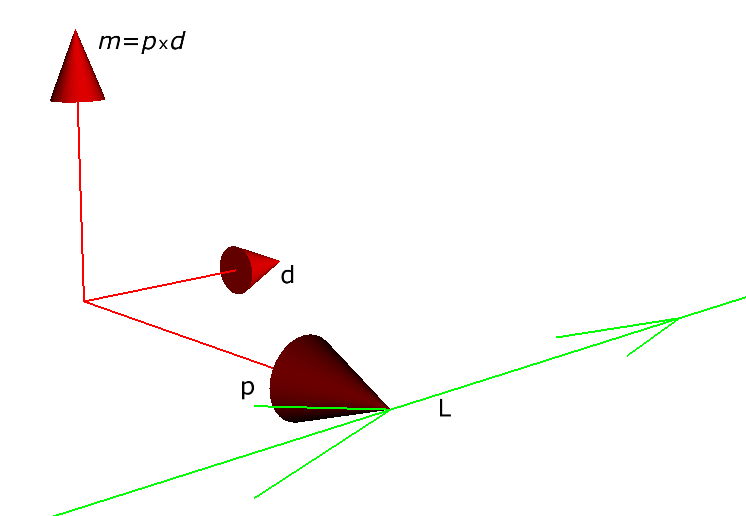
\includegraphics[width=0.6\textwidth]{linedef}
    }
  \end{center}
\end{figure}

In the homogeneous model, the line through weighted points $p = \lambda_p (\ez + \V{p})$ and $q = \lambda_q (\ez + \V{q})$ with weight $\lambda_p \lambda_q$ is represented as 
\begin{align*} 
  L &= p \wedge q \\
  &= (\lambda_p \ez) \wedge (\lambda_q \V{q}) + (\lambda_p \V{p}) \wedge (\lambda_q \ez) + (\lambda_p \V{p}) \wedge (\lambda_q \V{q}) \\
  &= \lambda_p\lambda_q (\ez \wedge (\V{q} - \V{p}) + \V{p} \wedge \V{q}) ,
\end{align*}
with the following dependency relationship: 
\begin{equation} \label{eq:gaplucker0} 
  \pluckerid(L) = \lambda_p \lambda_q (\ez \wedge (\V{q} - \V{p}) \wedge (\V{p} \wedge \V{q})) = 0 .
\end{equation}

Through this relation, the 8 parameters of this representation (3 for \V{p}, 3 for \V{q}, 1 for $\lambda_p$ and 1 for $\lambda_q$) have only 5 degrees of freedom.  

The classical parameters to characterize a line, its direction and moment, are easily recognized in this expression.  The direction $\V{d} = \V{p} - \V{q}$ is encoded in the first factor as $\ez \wedge -\V{d} = \V{d} \wedge \ez = \V{d} \ez$.  
The moment $\V{m} = \V{p} \times \V{q} = \edual{(\V{p} \wedge \V{q})}$ can be found in the second term as $\eundual{\V{m}} = \eundual{(\edual{(\V{p} \wedge \V{q})})} = \V{p} \wedge \V{q}$, which results in another general formula for lines:
\begin{equation*}
  L = \V{d} \ez + \eundual{\V{m}}.
\end{equation*}

Within classical literature of linear algebra, the same object is written as $-\plucker{\V{d}}{\V{m}}$, using Pl\"ucker coordinates to denote a line as a 6D vector.  The constraint of \autoref{eq:gaplucker0} is expressed as 
\begin{equation} \label{eq:laplucker0}
  \pluckerid(L) = \V{d} \dotp \V{m} = 0 .
\end{equation}

The relation from \autoref{eq:gaplucker0} and \autoref{eq:laplucker0} are indeed equal:
\begin{align*}
  \ez \wedge (\V{q} - \V{p}) \wedge (\V{p} \wedge \V{q}) 
  &= \ez \wedge \V{d} \wedge (\eundual{\V{m}}) \\
  &= \V{d} \wedge (\eundual{\V{m}}) \\
  &= \V{d} \dotp \edual{(\eundual{\V{m}})} \\
  &= \V{d} \dotp \V{m} .
\end{align*}
Pottmann and Wallner show this as well~\cite[Lemma 2.1.2]{Pottmann}, and name this relationship the Pl\"ucker identity.

The set of 6D vectors $-\plucker{\V{d}}{\V{m}}$ that comply with this constraint corresponds to the points on the Klein quadric.

The Pl\"ucker coordinates of a line are often treated as just six slots for storing numbers.  In most cases, operations on these elements are defined to manipulate two 3D vectors, \V{d} and \V{m}, instead of the whole 6D element.  

Because of this, the user is often unaware of most of the algebraic structure.  In fact, this 6D vector corresponds to
\begin{equation*}
  L = d_1 \ez\ee + d_2 \ez\et + d_3 \ez\ed + m_1 \et\ed + m_2 \ed\ee + m_3 \ee\et .
\end{equation*}

The set $\{\ez\ee, \ez\et, \ez\ed, \et\ed, \ed\ee, \ee\et\}$ forms an orthogonal and complete basis of the bivectors of the homogeneous model of $\reals^3$ with inner product $\ez^2 = \ee^2 = \et^2 = \ed^2 = 1$\footnote{The homogeneous model does not have a natural metric.  Some sources choose for $\ez^2 = -1$, while others work with $\ez^2 = 1$.  Its inverse depends on this definition; $\inverse{\ez} = -\ez$ if $\ez^2 = -1$.  With our chosen metric, $\inverse{\ez} = \ez$.}.  The basis is orthogonal, because for any two elements $E_1, E_2$ it holds that $E_1 \lcont E_2 = 0$. It is also complete; it contains $(^4_2) = 6$ linear independent elements.

The Pl\"ucker model uses these six elements as its basis; it treats these bivectors as 1-dimensional elements.  These elements will be known as $\{\eze, \ezt, \ezd, \etd, \ede, \eet\}$.  Li and Zhang~\cite{Hongbo} define an embedding from the Pl\"ucker model to the homogeneous model:\footnote{This definition of the embedding function $\Em$ is not the same as the one given by the internal report~\cite{internal}.  The internal report defines its inverse, from the homogeneous model to the Pl\"ucker model.}
\begin{equation} \label{eq:Em}
  \Em(A) = \left\{ 
    \begin{array}{ll}
      \ez \wedge \V{e}_i &\mbox{if $A = e_{0i}$}; \\
      \V{e}_i \wedge \V{e}_j &\mbox{if $A = e_{ij}$}; \\
      \Em(B) + \Em(C) &\mbox{if $A = B + C$}; \\
      \Em(B) \wedge \Em(C) &\mbox{if $A = B \wedge C$}; \\
      \left[\Em(B) \wedge \Em(C)\right] &\mbox{if $A = B \lcont C$}. \\
    \end{array}
    \right.
\end{equation}
In the last line, the inner product for the Pl\"ucker model is defined.  The bracket returns the proportionality factor of $\Em(y) \wedge \Em(z)$ to the homogeneous pseudoscalar $\hpseudo$.  Giving the homogeneous space metric structure $\reals^{4,0}$, the bracket construction is the same as dualization with respect to the pseudoscalar.  This metric gives the multiplication table of \autoref{tab:nullmetric}.  Because each of its basis elements correspond to a null vector, this basis is called the null basis.  Li and Zhang show that each null vector of this space satisfies the Pl\"ucker identity, and thus correspond to a line.  Let $a$ be a vector in this model.  $a$ is a line if and only if

\begin{align*}
  \Em(a \dotp a) &= \left[\Em(a) \wedge \Em(a)\right] \\
    &= \left[ 2 \left( a_{01} a_{23} \ez\ee \wedge \et\ed + a_{02} a_{31} \ez\et \wedge \ed\ee + a_{03} a_{12} \ez\ed \wedge \ee\et \right) \right] \\
    &= 2 \left( a_{01} a_{23} + a_{02} a_{31} + a_{03} a_{12} \right) \\
    &= 2 (a_{01} \ee + a_{02} \et + a_{03} \ed) \dotp (a_{23} \ee + a_{31} \et + a_{23} \ed) \\
    &= 2 \V{d} \dotp \V{m} \\ 
    &= 2 \pluckerid(A),
\end{align*}
with $A = \plucker{\V{d}}{\V{m}}$ the corresponding Pl\"ucker coordinate representation of $a$.

\begin{table}[t]
  \caption{The multiplication table of the inner product for the Pl\"ucker model on the null basis.}
  \label{tab:nullmetric}
  \begin{center}
    \begin{tabular}{|c||c|c|c|c|c|c|}
      \hline
      $\dotp$ & $\eze$ & $\ezt$ & $\ezt$ & $\etd$ & $\ede$ & $\eet$ \\
      \hline \hline
      $\eze$ & 0 & 0 & 0 & 1 & 0 & 0 \\
      \hline
      $\ezt$ & 0 & 0 & 0 & 0 & 1 & 0 \\
      \hline
      $\ezd$ & 0 & 0 & 0 & 0 & 0 & 1 \\
      \hline
      $\etd$ & 1 & 0 & 0 & 0 & 0 & 0 \\
      \hline
      $\ede$ & 0 & 1 & 0 & 0 & 0 & 0 \\
      \hline
      $\eet$ & 0 & 0 & 1 & 0 & 0 & 0 \\
      \hline
    \end{tabular}
  \end{center}
\end{table}

Li and Zhang also show that the 6D space has the metric structure of $\reals^{3,3}$.  To demonstrate this structure, we give a second basis:

\begin{equation*}
  \begin{split}
  \left\{\ap, \bp, \cp, \am, \bm, \cm\right\} =
    & \left\{ \frac{\eze + \etd}{\sqrt{2}}, \frac{\ezt + \ede}{\sqrt{2}}, \frac{\ezd + \eet}{\sqrt{2}}, \right.\\
    & \left.  \frac{\eze - \etd}{\sqrt{2}}, \frac{\ezt - \ede}{\sqrt{2}}, \frac{\ezd - \eet}{\sqrt{2}}, \right\}
.
\end{split}
\end{equation*}

Without changing the semantics of the inner product, we obtain the multiplication table of \autoref{tab:screwmetric}.  It is apparent that the metric structure is $\reals^{3,3}$; three basis vectors, $\ap, \bp, \cp$, square to $1$, while the other three basis vectors, $\am, \bm, \cm$ square to $-1$.  

\begin{table}[t]
  \caption{The multiplication table of the inner product for the Pl\"ucker model on the screw basis.}
  \label{tab:screwmetric}
  \begin{center}
    \begin{tabular}{|c||c|c|c|c|c|c|}
      \hline
      $\dotp$ & $\ap$ & $\bp$ & $\cp$ & $\am$ & $\bm$ & $\cm$ \\
      \hline \hline
      $\ap$ & 1 & 0 & 0 & 0 & 0 & 0 \\
      \hline
      $\bp$ & 0 & 1 & 0 & 0 & 0 & 0 \\
      \hline
      $\cp$ & 0 & 0 & 1 & 0 & 0 & 0 \\
      \hline
      $\am$ & 0 & 0 & 0 & -1 & 0 & 0 \\
      \hline
      $\bm$ & 0 & 0 & 0 & 0 & -1 & 0 \\
      \hline
      $\cm$ & 0 & 0 & 0 & 0 & 0 & -1 \\
      \hline
    \end{tabular}
  \end{center}
\end{table}

It is also clear that the basis elements do not represent lines, as no basis vector squares to $0$.  \Autoref{ch:research} demonstrates that all non-null vectors of the Pl\"ucker model represent screw axes.  

This screw basis is good to demonstrate the metric structure of the model.  However, the null basis makes the connection to the homogeneous model more transparant.  

\subsubsection{Intersecting lines}
The classical approach of linear algebra~\cite{Shoemake} gives a formula to test if two lines $L_1 = -\plucker{\V{d}_1}{\V{m}_1}, L_2 = -\plucker{\V{d}_2}{\V{m}_2}$ are coplanar: $\V{d}_1 \dotp \V{m}_2 + \V{d}_2 \dotp \V{m}_1 = 0$.  This expression can be translated to our model:

\begin{align}
  \label{eq:coplanar}
  0 &= \V{d}_1 \dotp \V{m}_2 + \V{d}_2 \dotp \V{m}_1 \nonumber \\
    &= \left( d_{1,1} m_{2,1} + d_{1,2} m_{2,2} + d_{1,3} m_{2,3} \right) + \left( d_{2,1} m_{1,1} + d_{2,2} m_{1,2} + d_{2,3} m_{1,3} \right) \nonumber \\
    &= d_{1,1} m_{2,1} + d_{1,2} m_{2,2} + d_{1,3} m_{2,3} + m_{1,1} d_{2,1} + m_{1,2} d_{2,2} + m_{1,3} d_{2,3} \nonumber \\
    &= d_{1,1} \eze \dotp m_{2,1} \etd + d_{1,2} \ezt \dotp m_{2,2} \ede + d_{1,3} \ezd \dotp m_{2,3} \eet \nonumber \\
    &\quad + m_{1,1} \etd \dotp d_{2,1} \eze + m_{1,2} \ede \dotp d_{2,2} \ezt + m_{1,3} \eet \dotp d_{2,3} \ezd \nonumber \\
    &= \Em^{-1}\left( \V{d}_1\ez + \eundual{\V{m}_1} \right) \dotp \Em^{-1}\left( \V{d}_2\ez + \eundual{\V{m}_2} \right) \nonumber \\
    &= l_1 \dotp l_2,
\end{align}
with $l_1, l_2$ the null vectors of the Pl\"ucker model corresponding to $L_1, L_2$.  This test for coplanarity is a projective interpretation of intersection.  That is, even two parallel lines have an intersection.  This ``point'' of intersection $\V{p}$ is at infinity, and $\V{p} \dotp \ez = 0$.  Projectively, points at infinity are not any different from other points.

  This test for intersection also gives a geometric interpretation to the inner product of the Pl\"ucker model.

The point of intersection itself cannot easily be computed in the Pl\"ucker model, as it has no direct representation of points.  Therefore, we will use the embedding function to the homogeneous model.  This lets us compute the point of intersection by the meet of $\Em(l_1)$ and $\Em(l_2)$~\cite[Section 11.7.1]{TheBook}:
\begin{align}
  \label{eq:intersect}
  p =& \Em\left(l_1\right) \cap \Em\left(l_2\right) \nonumber \\
  =& \undual{\left(\dual{\Em\left(l_2\right)} \wedge \dual{\Em\left(l_1\right)}\right)} .
\end{align}

This works for the cases of intersecting in both finite and infinite points; infinite points in the homogeneous model are represented as purely Euclidean vectors.

Together with the test for coplanarity, this can be used to see if two lines are parallel: $(l_1 \dotp l_2) (p \dotp \ez) = 0$.  In classical literature~\cite{Shoemake}, one finds a similar test, although both lines need to be decomposed into their direction and moment vectors:
\begin{align*}
  0 &= \V{d}_1 \times \V{d}_2 \\
    &= \left( \V{d}_1 \V{d}_2 \right) \lcont \epseudo .
\end{align*}
